\documentclass{beamer}

\mode<presentation>
{
  \usetheme{CambridgeUS}
  \setbeamercovered{transparent}
}

\usepackage[english]{babel}
\usepackage[latin1]{inputenc}
\usepackage{times}
\usepackage[T1]{fontenc} 
% Or whatever. Note that the encoding and the font should match. If T1
% does not look nice, try deleting the line with the fontenc.
\usepackage{amsmath}

\newcommand{\linespace}{\vskip 0.25cm}

% The text in square brackets is the short version of your title and will be used in the
% header/footer depending on your theme.
\title[Graph database analysis of GP dynamics]{Silico-paleontology with graph databases}
%{Using Graph Databases to Explore Genetic Programming Run Dynamics}

% Sub-titles are optional - uncomment and edit the next line if you want one.
\subtitle{Rooting through the relics of digital evolution} 

% The text in square brackets is the short version of your name(s) and will be used in the
% header/footer depending on your theme.
\author[McPhee \& Donatucci (w/ Dramdahl)]{Nic McPhee \& David Donatucci \\ (w/ M. Kirbie Dramdahl)}

% The text in square brackets is the short version of your institution and will be used in the
% header/footer depending on your theme.
\institute[UMM]
{
  Division of Science and Mathematics \\
  University of Minnesota, Morris \\
  Morris, Minnesota, USA
}

% The text in square brackets is the short version of the date if you need that.
\date[May 2015, GPTP, Ann Arbor MI] % (optional)
{May 2015 \\ Genetic Programming Theory and Practice \\ University of Michigan \\ Ann Arbor, MI}

% Delete this, if you do not want the table of contents to pop up at
% the beginning of each subsection:
\AtBeginSection[]
{
  \begin{frame}<beamer>
    \frametitle{Outline}
    \tableofcontents[currentsection, hideothersubsections]
  \end{frame}
}

\begin{document}

\begin{frame}
  \titlepage
\end{frame}

% For a 20-25 minute senior seminar talk you probably want something like:
% - Two or three major sections (other than the summary).
% - At *most* three subsections per section.
% - Talk about 30s to 2min per frame. So there should probably be between
%   15 and 30 frames, all told.

\section*{Overview}

\subsection*{The Big Picture}

\begin{frame}
  \frametitle{The Big Picture}
  
  \begin{itemize}
	\item Genetic programming clearly \emph{works}.
	\item But we rarely know \emph{why} or \emph{how}.
	\item Databases allow examination of the internal interactions of a run.
	\item Graph databases better suited for this than relational databases.
	\item Silico-paleontology can help us understand and improve our tools.
  \end{itemize}

\end{frame}

\subsection*{Outline}

\begin{frame}
  \frametitle{Outline}
  \tableofcontents[hideallsubsections]
\end{frame}

\section{What do we know? (And how do we talk about it?)}

\subsection{We throw so much away}

\begin{frame}{We keep/see/share so little}
	
	\begin{columns}
		\begin{column}{0.6 \linewidth}
			EC research has the potential to generate \emph{huge} amounts of data.
			\linespace
			What do we normally do with that data?
			\linespace
			We normally throw it away -- \& paleontologists weep!
			\linespace
			\includegraphics[width = 0.8 \linewidth]{Figures/FossilsMedium.jpg} \\
			\tiny{\url{https://www.flickr.com/photos/blmoregon/14566767645/}}
		\end{column}
		\begin{column}{0.4 \linewidth}
			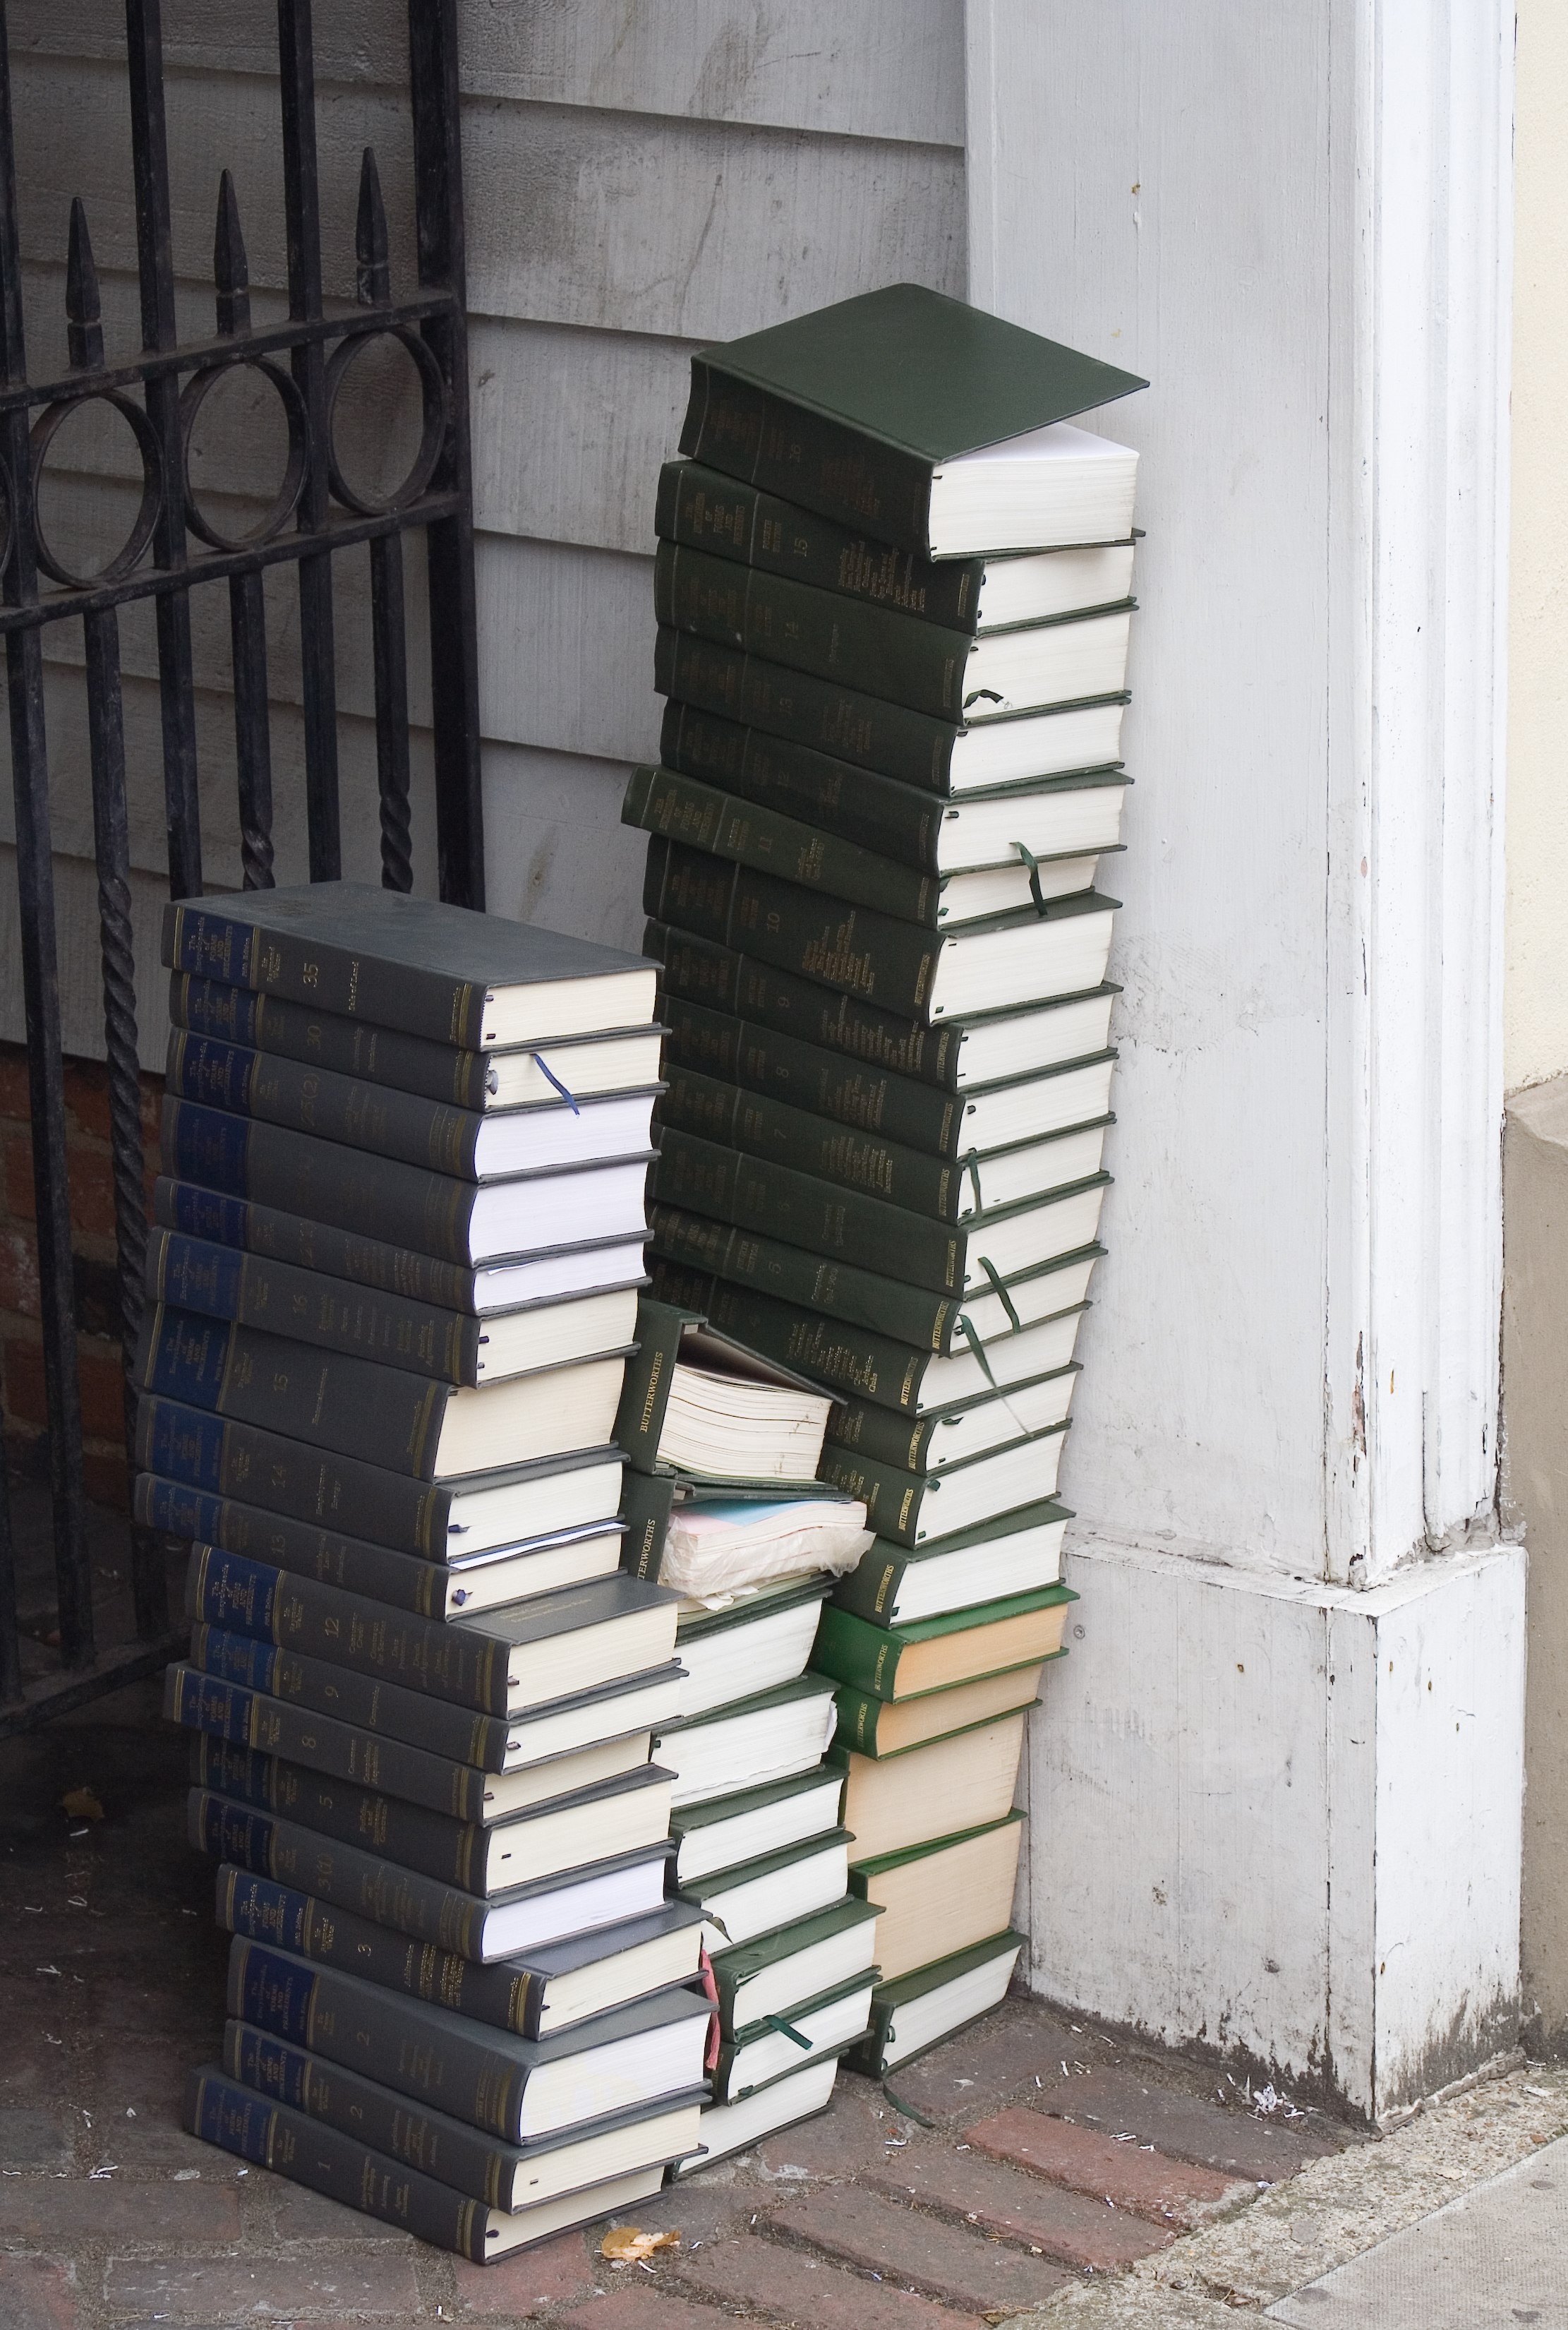
\includegraphics[height= 0.7 \textheight]{Figures/Abandoned_books.jpg} \\
			\tiny{\url{https://www.flickr.com/photos/nicmcphee/1323950471}}
		\end{column}
	\end{columns}
\end{frame}

\subsection{Summary results just summarize}

\begin{frame}{Oooh -- a table of results!}

\begin{columns}
	\begin{column}{0.4 \linewidth}
		\centering
\begin{tabular}{lrrr}
	& \multicolumn{3}{c}{Treatment} \\ \cline{2-4}
	\textbf{Problem} & \textbf{L} & \textbf{T} & \textbf{I} \\
	\hline
	RSWN & 55 & 13 & 17 \\
	SYL & 22 & 1 & 2 \\
	SLB & 75 & 19 & 10 \\
	NTZ & 57 & 15 & 7
\end{tabular}
\end{column}

\begin{column}{0.55 \linewidth}
	\begin{overprint}
		\onslide<1>
		These show successes on 4 problems for 3 different treatments
		\linespace
		L seems to be winning

		\onslide<2>
		But \emph{why?!?!?}		
		\linespace
		What's actually \emph{happening} in all those matings and crossovers and mutations that makes the difference?
	\end{overprint}
\end{column}
\end{columns}
\end{frame}

\subsection{Plots are better (but can still obscure details)}

\begin{frame}{Let's draw pretty pictures}
	
	\begin{columns}
		\begin{column}{0.55 \linewidth}
			\centering
			\includegraphics[width = \linewidth]{Figures/rswn_diversity.pdf}
		\end{column}
		
		\begin{column}{0.4 \linewidth}
			\begin{overprint}
				\onslide<1>
				So much more data!
				\linespace
				Diversity over time across all the runs.
				\linespace
				L's diversity (top) is consistently higher than T (bottom).
				\linespace
				That might be important (and supports some hypotheses).
				
				\onslide<2>
				Still, this mushes all the runs together.
				\linespace
				And that likely obscures interesting things.
			\end{overprint}
		\end{column}
	\end{columns}
\end{frame}

\subsection{Can we zoom in to individual runs?}

\begin{frame}{Zooming in}
	
	\begin{columns}
		\begin{column}{0.55 \linewidth}
			\centering
			\includegraphics[width = \linewidth]{Figures/run6_lexicase_rswn_diversity.pdf}
		\end{column}
		
		\begin{column}{0.4 \linewidth}
			\begin{overprint}
				\onslide<1>
				Focusing on one successful L run now.
				\linespace
				Three big diversity changes:
				\begin{itemize}
					\item First 15 generations have a sharp drop then steep rise
					\item Around generation 40 a sharp drop and rise
					\item Sharp drop at end just before a solution is found
				\end{itemize}
				
				\onslide<2>
				\emph{What's happening at those sections of the run?}
				\linespace
				We want to be able to dig through a run and see what happened.
			\end{overprint}
		\end{column}
	\end{columns}
\end{frame}

\section[Using a graph DB]{Using a graph database}

\subsection{Goals}

\begin{frame}{Goals}
	\begin{columns}
		\begin{column}{0.6 \linewidth}
					We want to store and analyze \emph{all} the individuals and their relationships.
					\linespace
					Ancestry relationships are naturally modeled with a graph
					\linespace
					So graph databases seem a natural tool for the relationship part.
					\linespace
					\centering
					\includegraphics[width=0.8 \linewidth]{Figures/FamilyTree.jpg} \\
					\tiny{\url{https://www.flickr.com/photos/herry/3228640890}}
		\end{column}
		\begin{column}{0.4 \linewidth}
			\includegraphics[height= 0.75 \textheight]{Figures/HeuristicLabGraph.pdf} \\
			\tiny{\cite{Burlacu:2013:VGL:2464576.2482714}}
		\end{column}		
	\end{columns}
\end{frame}

\subsection{Neo4j}

\begin{frame}
	\frametitle{Neo4j}
	
	
	
\begin{columns} 
\begin{column}{0.60 \textwidth}
Neo4j is a graph database.
		\begin{itemize}
		\item relatively new tool
			\begin{itemize}
			\item initial release 2007
			\item popularized in 2010
			\end{itemize}
		\item information is stored using a graph
		\item nodes and relationships
		\item efficient recursive queries compared with traditional databases
		\end{itemize}
		\end{column}
		\begin{column}{0.40\textwidth}
   % \includegraphics[width=0.95\textwidth]{graphdb-neo4j.png}
       \\
    \only{\tiny{Neo4j \ \url{http://goo.gl/nzRWSV}}}
  \end{column}
  \end{columns}

\end{frame}

\subsection{Cypher}

\begin{frame}
	\frametitle{Cypher}
	Neo4j's query language is Cypher.
	\begin{columns}
	\begin{column}{0.40\textwidth}

	Fundamental elements of Cypher queries:
		\begin{itemize}
		\item START
		\item RETURN
		\item MATCH
		\item WHERE
		\end{itemize}
	\end{column}
	\begin{column}{0.60\textwidth}

	% \includegraphics[width=.95\textwidth]{parents.pdf}
	%\linebreak
	\emph{
START parent=node(43)
\linebreak
MATCH (parent)-[:PARENTOF]->(child)
\linebreak
\textbf{WHERE id(child) < 47}
\linebreak
RETURN parent, child;
}

	\end{column}	
	\end{columns}
\end{frame}

\section[Setup]{Experimental Setup}

\subsection{Configurations}

\begin{frame}
\frametitle{Run Configurations}
\begin{description}[align=left, leftmargin=*]
{\small
\item[Target Function] sin(x)
\item[Variables] x (range 0.0 to 6.2, incremented by steps of 0.1)
\item[Constants] range between -5.0 and 5.0
\item[Operations] addition (+), subtraction (-), multiplication (*), protected division (/)
\item[Generation Number] 100
\item[Population Size Per Gen] 1,000 (3 runs) and 10,000 (1 run)
\item[Transform Percentages] crossover (90\%), mutation (1\%), reproduction (9\%)
\item[Elitism] best 1\%
\item[Fitness] absolute error between target function and individual function
}
\end{description}
\end{frame}

\section[Results]{Results}

\subsection[Questions Asked]{Questions Asked}

\begin{frame}
\frametitle{Questions Asked}
\begin{enumerate}
\item \emph{What does the fitness of the ``winning'' individual's ancestry line look like over time?}
\item \emph{How often does mutation improve fitness? Also, how often does crossover improve fitness, where the root parent is more fit than the non-root parent, and vice versa?}
\item \emph{Does a group of individuals have a common root parent ancestor and what is the latest generation where such an ancestor occurs?}
\item \emph{How many individuals in the initial generation have any root parent descendants in the final generation?}
\end{enumerate}
\end{frame}

\subsection[Fitness Graph]{Fitness Over Time}

\begin{frame}
\frametitle{Fitness Over Time}
\emph{What does the fitness of the ``winning'' individual's ancestry line look like over time?}
\begin{center}
% \includegraphics[width=0.85\textwidth]{Combined_fitness_over_time_no_dashed}
\end{center}
\end{frame}

\subsection[Improved Transformations]{Improved Transformations}

\begin{frame}
\frametitle{Percentage of Improved Transformations}
\emph{How often does mutation and crossover improve fitness?}
\begin{center}
{\tiny Results for Three 1,000 Individual Runs and One 10,000 Individual Run}
% \includegraphics[width=0.95\textwidth]{All_percentages_over_time}
\end{center}
\end{frame}

\subsection[Common Ancestor]{Common Ancestor}

\begin{frame}
\frametitle{Common Ancestor}
\emph{Does a group of individuals have a common root parent ancestor and how many initial generation individuals have descendants in the final generation?}
\begin{center}
% \includegraphics[height=0.70\textheight]{subset_confluence_trimmed}
\end{center}

\end{frame}

\section[Conclusions]{Conclusions}

\begin{frame}
\frametitle{Conclusions}

\begin{itemize}
\item We can gather internal data efficiently.
\item Provides more in depth information than statistical summaries. 
\item Support for hypotheses.
\end{itemize}
\linespace
\linespace
\linespace
\linespace

Future Work
\begin{itemize}
\item Trying different setup configurations.
\item Enforcing the root parent to have better fitness in XO.
\item Dynamically change parameters.
\end{itemize}
\end{frame}

\begin{frame}
	\frametitle{Thanks!}
	
	Thank you for your time and attention!
		
	\linespace
	\linespace
	
	Contacts:  
	\begin{itemize}
		\item \texttt{donat056@morris.umn.edu}
		\item \texttt{dramd002@morris.umn.edu}
		\item \texttt{mcphee@morris.umn.edu}
	\end{itemize}
	
	\linespace
	\linespace
	
	\begin{center}
	{\huge Questions?}
	\end{center}
\end{frame}

\section*{References}

\begin{frame} 
\frametitle{References}
% \nocite{*}
\bibliographystyle{alpha}
{\tiny \bibliography{GraphDBandGP}}
\end{frame} 

\end{document}


